%% Do not edit unless you really know what you are doing.
\documentclass[twoside,english]{report}
\usepackage[sc]{mathpazo}
\usepackage[scaled=0.9]{helvet}
\renewcommand{\ttdefault}{lmtt}
\usepackage[T1]{fontenc}
\usepackage[latin9]{inputenc}
\usepackage[a4paper]{geometry}
\geometry{verbose,lmargin=2cm,rmargin=2cm}
\usepackage{fancyhdr}
\pagestyle{fancy}
\setcounter{secnumdepth}{3}
\setcounter{tocdepth}{3}
\setlength{\parskip}{\smallskipamount}
\setlength{\parindent}{0pt}
\usepackage{babel}
\usepackage{nomencl}
% the following is useful when we have the old nomencl.sty package
\providecommand{\printnomenclature}{\printglossary}
\providecommand{\makenomenclature}{\makeglossary}
\makenomenclature
\usepackage[unicode=true,
 bookmarks=true,bookmarksnumbered=false,bookmarksopen=false,
 breaklinks=false,pdfborder={0 0 1},backref=false,colorlinks=false]
 {hyperref}
\usepackage{breakurl}

%%COMMENTARE PRIMA DI PUBBLICARE 
%----------------------------------------------------------------
%\usepackage{draftwatermark} %per il watermark sullo sfondo
%----------------------------------------------------------------
% Per mettere dei commenti per revisione si possono usare i comandi:
% \unsure per le parti in cui non si � sicuri
% \change per le parti che devono essere cambiate in fase di revisone
% \improvement per le parti che devono essere descritte meglio
% \info per scrivere un commento informativo
% \thiswillnotshow � un commento che viene visto solo nel punto in cui viene piazzato e non nella lista delle note
%----------------------------------------------------------------

\makeatletter


% Customization file for the titlepage and document
%************************************************************
% Required stuff
%************************************************************
\usepackage{graphicx}
\usepackage{euler}
\usepackage[detect-all]{siunitx}
\usepackage{sectsty}
\usepackage[font={footnotesize }]{caption}
\usepackage{multicol}
\usepackage{prettyref}

\usepackage{listings}

\allsectionsfont{\rmfamily}

% Page customization
\usepackage{fancyhdr}
\pagestyle{fancy}

% Color
\usepackage{color}
\definecolor{light-gray}{gray}{0.85}
\definecolor{dark-gray}{gray}{0.75}

\fancyhead{}  % clear all header fields
\fancyhead[LO,RE]{\rule[-2ex]{0pt}{2ex}\fontsize{9}{11} \selectfont \myPhase}
\fancyhead[RO,LE]{\raisebox{-0.35cm}{
\includegraphics[height=1.2cm,keepaspectratio]{gfx/Logo_TotalBlack.pdf}}}
\fancyhead[CO,CE]{\fontsize{9}{11} \selectfont \myIPT}
\fancyfoot{}  % clear all footer fields
\fancyfoot[RO,LE]{\fontsize{5.5}{8} \selectfont This work is to be considered classified. The use is allowed only for Skyward Experimental Rocketry related activities and projects. For public access please contact \href{mailto:info@skywarder.eu}{info@skywarder.eu}}
\fancyfoot[RE,LO]{\fontsize{9}{11} \selectfont \thepage}
\fancyheadoffset[LE,RO]{0.2pt}
\renewcommand{\headrulewidth}{0.2pt}
\renewcommand{\footrulewidth}{0.2pt}
\renewcommand{\headrule}{\hbox to\headwidth{%
   \leaders\hrule height \headrulewidth\hfill}}
\renewcommand{\footrule}{\hbox to\headwidth{%
    \leaders\hrule height \headrulewidth\hfill}}
\hypersetup{colorlinks=true, linkcolor=blue ,linktoc=page,citecolor=black}

\usepackage{pdfpages} %per includere pdf di più pagine


% Custom notes
\usepackage{xargs}                      % Use more than one optional parameter in a new commands
\usepackage[pdftex,dvipsnames]{xcolor}  % Coloured text etc.

\usepackage[colorinlistoftodos,prependcaption,textsize=tiny]{todonotes}

\usepackage{nameref}

\newcommandx{\unsure}[2][1=]{\todo[linecolor=red,backgroundcolor=red!25,bordercolor=red,#1]{#2}}
\newcommandx{\change}[2][1=]{\todo[linecolor=blue,backgroundcolor=blue!25,bordercolor=blue,#1]{#2}}
\newcommandx{\info}[2][1=]{\todo[linecolor=OliveGreen,backgroundcolor=OliveGreen!25,bordercolor=OliveGreen,#1]{#2}}
\newcommandx{\improvement}[2][1=]{\todo[linecolor=Plum,backgroundcolor=Plum!25,bordercolor=Plum,#1]{#2}}
\newcommandx{\thiswillnotshow}[2][1=]{\todo[disable,#1]{#2}}
\reversemarginpar
\setlength{\marginparwidth}{2cm}
%End custom notes


%************************************************************
% Redefining numbering for sections
%************************************************************
%\renewcommand*\thesection{\arabic{section}}

%************************************************************
% Cross reference set-up
%************************************************************
\newrefformat{tab}{Table\,\ref{#1}}
\newrefformat{fig}{Figure\,\ref{#1}}
\newrefformat{eq}{Eq.\,\textup{(\ref{#1})}}
\newrefformat{sec}{Sec.\,\ref{#1}}
\newrefformat{sub}{Sec.\,\ref{#1}}

%************************************************************
% Fancy stuff
%************************************************************
\newcommand{\titlecap}[1]{\Huge{\textrm{#1}}}
\newcommand{\subtitlecap}[1]{\Large{\textsc{#1}}}
\newcommand{\sscap}[1]{\textbf{#1}}
\newcommand{\strong}[1]{\textbf{#1}}
\setlength{\headheight}{60pt} %%or

%************************************************************
% Helpful stuff to modify here, not in the LyX Document
%************************************************************
\newcommand{\myDate}{\today}
\newcommand{\myGroup}{Skyward Experimental Rocketry}
\newcommand{\myUrl}{\url{http://www.skywarder.eu}}
\newcommand{\myUni}{Politecnico di Milano}

\newcommand{\myPhase}{}
\newcommand{\myProject}{Entry Project 2020}
\newcommand{\myRevision}{0}
\newcommand{\myIPT}{Software \& Control Systems Team}
\newcommand{\myTitle}{Matlab Sensor Model}
\newcommand{\myAuthor}{Jan H\"ammelmann}
\newcommand{\myEditor}{}
\newcommand{\myEmail}{jan.hammelmann@skywarder.eu}

\newcommand{\mail}[1]{\href{mailto:#1}{\texttt{#1}}}

\makeatother

\begin{document}
\thispagestyle{empty}
\pdfbookmark{Titlepage}{Titlepage}

\vspace{3cm}
\begin{center}
\bigskip
\Large{\myDate}
\vspace{0.5cm}

%{
\titlecap{\myProject} \\
%\vspace{0.3cm}
%\titlecap{\myPhase}}\\
\vspace{0.4cm}
\rule{\linewidth}{0.5mm}
\titlecap{\myTitle}\\
\vspace{0.4cm}
\titlecap{REV. \myRevision}
\end{center}

\vfill
\begin{multicols}{2}
\centering{

\includegraphics[height=4cm]{gfx/Logo_Colour.pdf} \\

\includegraphics[height=3cm]{gfx/Logo_Polimi}
}
\vfill
\columnbreak
{\centering{
	\subtitlecap{\myIPT} \\
	\vspace{0.7em}
	\normalsize
	\textrm{\myGroup \\
	\myUni }}}
\vfill

\raggedright{\textbf{Author}: {\myAuthor}\\
\textbf{Editor}: {\myEditor}}

						
\end{multicols}

\clearpage

%*******************************************************
% Titleback
%*******************************************************
\thispagestyle{empty}

\hfill
\vspace{5cm}

\strong{Abstract}\\
Scrivi qui il tuo abstract
\vfill

\begin{multicols}{2}
\medskip
\noindent{\sscap{Website}}: \\
\url{http://www.skywarder.eu}


\medskip
\noindent{\sscap{E-mail}}: \\
\mail{\myEmail}
\vfill
\columnbreak
\section*{Restricted use policy}
\fontsize{8}{11} \selectfont This report is developed during the activities done within Skyward Experimental Rocketry association. Its use is allowed only for Skyward Experimental Rocketry related purposes. If you're a Skyward member, please don't send or release publicly this file without previous acceptance from Direction Board.
For public access and publication please contact \href{mailto:info@skywarder.eu}{info@skywarder.eu}.
\end{multicols}
\vspace{1cm}
\hrule
\bigskip
\clearpage


\pagenumbering{roman}

\begin{multicols}{2}

\printnomenclature{}

\end{multicols}

\tableofcontents{}

\listoffigures


\listoftables

%%COMMENTARE PRIMA DI PUBBLICARE 
%----------------------------------------------------------------
\listoftodos[Notes] %per avere l'elenco delle note
%----------------------------------------------------------------

\clearpage{}

\pagenumbering{arabic}

\setcounter{page}{1}

\global\long\def\diff{\text{d}}


\chapter*{Change Log}
\setlength{\tabcolsep}{0.5em} % for the horizontal padding
{\renewcommand{\arraystretch}{2}% for the vertical padding
	\begin{table}[h]
		\centering
		%\resizebox{\textwidth}{!}
	\end{table}


\chapter{Introduction}
In this entry project of 2020 classes should be programmed, which that simulates the acquisition process of real sensors with all the non idealities it leads to. The programming style should be object oriented . After creating the object of the classes should be initialized, which represent the real used sensors of the rocket project.

In the following chapters the implemented classes, the used sensor and the defined properties are described.

\chapter{Implementation}
The project is separated in small parts. With the function \verb|createMagneticData(magneticDensity, q0, q1, q2, q3)| magnetic data can be created from the quaternion states of the simulator. Afterwards the sensor data can be manipulated the \verb|sens| method of the implemented sensors. For the implementation, depending on the type of sensor the classes Sensor, Sensor3D or GPS can be used. In this project some sensors where already initialized in the \verb|initSensor.m| script.

\section{Classes}
\subsection{Sensor}
Sensor is inheriting from handle to be able to change the properties inside methods. The properties of the class are:
\begin{lstlisting}
	minMeasurementRange; % Max limit of sensor
	maxMeasurementRange; % Min limit of sensor
	
	resolution; % resolution of the sensor
	
	noiseVariance; % Varianze for the gaussian white noise
	
	offset; % Offset in all directions
	
	tempOffset; % Coefficent for temperature depending offset
	
	dt; % Sampling time
	
	error2dOffset; % first column: inputArg, second column: relativeArg, third column: error
\end{lstlisting}

They are needed to use the methods of the class. With the method \verb|sens(inputArg,temp)| all following methods are called where the necessary properties are defined. The sensor class is created for 1D sensors. Now the methods called in the sens method are shortly described.

\subsubsection{saturation} \label{subsub:saturation}
This method limits inputArg to the properties minMeasurementRange at the lower end and maxMeasurementRange at the upper end.


\subsubsection{quantization} \label{subsub:quantization}
This method gets the input inputArg and quantized this with the property resolution. 


\subsubsection{whiteNoise} \label{subsub:whiteNoise}
This method adds to the input inputArg a gaussian white noise with the variance of the property noiseVariance.


\subsubsection{add2DOffset} \label{sub:add2DOffset}
The method takes the inputs inputArg and temp and uses the property error2dOffset of the object, which has to be defined before the use of the method. Add2DOffset interpolates between the data points of the 2D dataset error2dOffset [x1,x2,y] and finds a value yq that fits to the inputs inputArg and temp which refer to x1 and x2. Value yq is then added to inputArg and results in outputArg.


\subsubsection{addOffset} \label{subsub:addOffset}
Adds the properties offset to the input signal.

\subsubsection{addTempOffset} \label{subsub:addTempOffset}
Adds the property tempOffset multiplied by the temperature input temp to the input signal.


\subsection{Sensor3D}
Sensor is inheriting form Sensor.

The properties of the class are:
\begin{lstlisting}
	offsetX; % offset in x direction
	offsetY; % offset in y direction
	offsetZ; % offset in z direction
	
	walkDiffusionCoef; % diffusion coefficient for the random walk
	
	transMatrix % transformation matrix
\end{lstlisting}

With the method \verb|sens(inputArgX,inputArgY,inputArgZ,temp)| all methods from class sensor are called for all three sensor axis plus the methods defined in class Sensor3D. The methods are addOffset3D, randomWalk and tranformAxis.

\subsubsection{addOffset3D} \label{subsub:addOffset3D}
Like the method addOffset in class Sensor this method is adding a offset independent to all three axis with the value of the properties offsetX, offsetY and offsetZ.

\subsubsection{randomWalk} \label{subsub:randomWalk}
This method is adding a Brown motion to the sensor data with the diffusion coefficient of the property walkDiffusionCoef.

\subsubsection{tranformAxis} \label{subsub:tranformAxis}
This method is transforming the input data vector with the transformation matrix in property transMatrix.

\subsection{GPS}
GPS is inheriting from Sensor3D. The \verb|sens(lat,lon,alt,temp)| is before calling the method \verb|sens(inputArgX,inputArgY,inputArgZ,temp)| of the superclass Sesnor3D transforming the latitude, longitude and altitude in x, y and z coordinates. After using the method of Sensor3D the data is transformed back into latitude, longitude and altitude.


\section{Sensor implementation}

The Sensor are initialized in \verb|initSensor.m|. The values can be fined in the data sheets. In the following subsection the initializations is described.

\subsection{LSM9DS1}

The LSM9DS1 is a IMU including an accelerometer, a magnetometer and a gyroscope. The sensor data can be found in \cite{LSM9DS1}. The accelerometer is sensing the x, y and z accelerations in \si{mg}. The gyroscope is sensing the angular velocities in \si{mdps}. The magnetometer is sensing the x, y and z magnetic field in \si{mgauss}.

\subsubsection{Accelerometer}

Here the accelerometer of the LSM9DS1 is described. The parameter are defined with:

\begin{lstlisting}
	ACCEL_LSM9DS1=Sensor3D(); % acceleration in mg
	ACCEL_LSM9DS1.maxMeasurementRange=16000; % 2000, 4000, 8000, 16000 in mg
	ACCEL_LSM9DS1.minMeasurementRange=-16000; % -2000, -4000, -8000, -16000 in mg
	ACCEL_LSM9DS1.resolution=0.732; % 0.061, 0.122, 0.244, 0.732 in mg 
	ACCEL_LSM9DS1.noiseVariance=4; % guess in mg
	ACCEL_LSM9DS1.offsetX=0; % +-90 in mg
	ACCEL_LSM9DS1.offsetY=0; % +-90 in mg
	ACCEL_LSM9DS1.offsetZ=0; % +-90 in mg
	ACCEL_LSM9DS1.walkDiffusionCoef=1; % guess
	ACCEL_LSM9DS1.dt=0.01; % sampling time
\end{lstlisting}


\subsubsection{Magnetometer}

Here the magnetometer of the LSM9DS1 is described. The parameter are defined with:

\begin{lstlisting}
	MAGN_LSM9DS1=Sensor3D(); % magnetic field in mgauss
	MAGN_LSM9DS1.maxMeasurementRange=16000; % 4000, 8000, 12000, 16000 in mgauss
	MAGN_LSM9DS1.minMeasurementRange=-16000; % -4000, -8000, -12000, -16000 in mgauss
	MAGN_LSM9DS1.resolution=0.58; % 0.14, 0.29, 0.43, 0.58 in mgauss
	MAGN_LSM9DS1.noiseVariance=2; % guess in mgauss
	MAGN_LSM9DS1.offsetX=0; % +-1000 in mgauss
	MAGN_LSM9DS1.offsetY=0; % +-1000 in mgauss
	MAGN_LSM9DS1.offsetZ=0; % +-1000 in mgauss
	MAGN_LSM9DS1.walkDiffusionCoef=1; % guess
	MAGN_LSM9DS1.dt=0.01; % sampling time
	MAGN_LSM9DS1.transMatrix=diag([1 1 1]); % axis transformation
\end{lstlisting}


\subsubsection{Gyroscope}

Here the gyroscope of the LSM9DS1 is described. The parameter are defined with:

\begin{lstlisting}
	GYRO_LSM9DS1=Sensor3D(); % angular rate in mdps
	GYRO_LSM9DS1.maxMeasurementRange=2000e3; % 245e3, 500e3, 2000e3 in mdps
	GYRO_LSM9DS1.minMeasurementRange=-2000e3; % -245e3, -500e3, -2000e3 in mdps
	GYRO_LSM9DS1.resolution=70; % 8.75, 17.5, 70 in mdps
	GYRO_LSM9DS1.noiseVariance=100; % guess in mdps
	GYRO_LSM9DS1.offsetX=0; % +-30e3 in mdps
	GYRO_LSM9DS1.offsetY=0; % +-30e3 in mdps
	GYRO_LSM9DS1.offsetZ=0; % +-30e3 in mdps
	GYRO_LSM9DS1.walkDiffusionCoef=1; % guess
	GYRO_LSM9DS1.dt=0.01; % sampling time
	GYRO_LSM9DS1.transMatrix=diag([1 1 1]); % axis transformation

\end{lstlisting}

\subsection{MS580301BA01}

The MS580301BA01 is a barometer. The sensor data can be found in \cite{MS580301BA01}. The measuring unit is \si{mbar}.

For the sensor saturation \ref{sub:saturation}, quantization \ref{sub:quantization} and white noise \ref{sub:whiteNoise} is implemented. Furthermore there is a deterministic error for the sensor dependency on the pressure and temperature. This is implemented with the add2DOffset method \ref{sub:add2DOffset}. The data sheet of the sensor provides us with the information in figure \ref{fig:barometer_error_p}. The information is extracted in \verb|.\data\char\MS580301BA01| in the CSV files \verb|ep\_p\_0.csv|, \verb|ep\_p\_25.csv|, \verb|ep\_p\_85.csv|, \verb|ep\_p\_85.csv| and \verb|ep\_p\_-40.csv|. They are combined in a matrix with columns [pressure p, temperature T, error pressure ep]. This matrix must be used as property \verb|error2dOffset| of the MS580301BA01 object.

\begin{figure}[h]
	\centering
	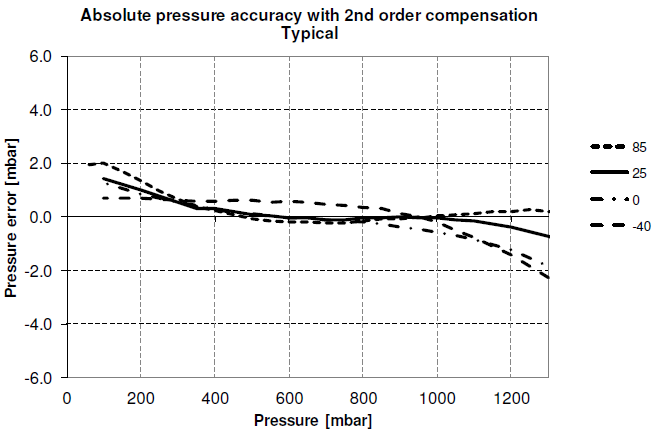
\includegraphics[scale=0.8]{images/barometer_error_p.PNG}
	\caption{Deterministic error of the barometer depending on pressure and temperature from \cite{MS580301BA01}}
	\label{fig:barometer_error_p}
\end{figure}

\subsubsection{Barometer}

Here the barometer MS580301BA01 is described. The parameter are defined with:

\begin{lstlisting}
	MS580301BA01=Sensor(); % presure in mbar, temp should be in C�
	MS580301BA01.maxMeasurementRange=1100; % 1100, 1300 in mbar
	MS580301BA01.minMeasurementRange=300; % 300, 10 in mbar
	MS580301BA01.resolution=0.065; % 0.012, 0.018, 0.027, 0.042, 0.065 in mbar
	MS580301BA01.noiseVariance=4; % guess in mbar
	MS580301BA01.error2dOffset=ep_data; % [p in mbar, T in celsius, ep in mbar]
\end{lstlisting}

\subsection{IIS2MDC}

The IIS2MDC is a magnetometer. The sensor data can be found in \cite{IIS2MDC}.

\subsubsection{Magnetometer}

Here the magnetometer IIS2MDC is described. The parameter are defined with:

\begin{lstlisting}
	MAGN_IIS2MDC=Sensor3D(); % magnetic field in mgauss, temp should be in C�-25C�
	MAGN_LSM9DS1.maxMeasurementRange=49152; % in mgauss
	MAGN_LSM9DS1.minMeasurementRange=-49152; % in mgauss
	MAGN_LSM9DS1.resolution=1.5; % in mgauss
	MAGN_LSM9DS1.tempOffset=0; % +-0.3 in mgauss
	MAGN_LSM9DS1.noiseVariance=9; % guess in mgauss
	MAGN_LSM9DS1.offsetX=0; % +-60 in mgauss
	MAGN_LSM9DS1.offsetY=0; % +-60 in mgauss
	MAGN_LSM9DS1.offsetZ=0; % +-60 in mgauss
	MAGN_LSM9DS1.walkDiffusionCoef=1; % guess
	MAGN_LSM9DS1.dt=0.01; % sampling time
	MAGN_LSM9DS1.transMatrix=diag([1 1 1]); % axis transformation
\end{lstlisting}

\subsection{NEO-M9N}

The NEO-M9N is a GPS module. The sensor data can be found in \cite{NEO-M9N}.

\subsubsection{GPS}

Here the magnetometer NEO-M9N is described. The parameter are defined with:

\begin{lstlisting}
GPS_NEOM9N=GPS(); % lon, in degree lat in deree, alt in m
GPS_NEOM9N.noiseVariance=4; % in m
GPS_NEOM9N.transMatrix=diag([1 1 1]); % axis transformation
\end{lstlisting}

\begin{thebibliography}{DOCUMENTI}
	\bibitem{LSM9DS1}
	LSM9DS1 data sheet
	
	\bibitem{MS580301BA01}
	MS580301BA01 data sheet
	
	\bibitem{IIS2MDC}
	IIS2MDC data sheet
	
	\bibitem{NEO-M9N}
	NEO-M9N data sheet
\end{thebibliography}

\end{document}
